\documentclass[12pt]{article}
\usepackage[utf8]{inputenc}
\usepackage[top=3cm, bottom=3cm, left=2cm, right=2cm]{geometry}
\usepackage{url}
\usepackage{color}
\usepackage{booktabs}
\usepackage{multirow}
\usepackage{todonotes}
\usepackage{tcolorbox}
\usepackage{graphicx}
\usepackage{hyperref}
\definecolor{SlateGray}{RGB}{112,128,144}
\definecolor{CeruleanBlue}{RGB}{42,82,190}
\definecolor{Coral}{RGB}{255,127,80}
\definecolor{PineGreen}{rgb}{0,0.5,0}
\definecolor{AmethystPurple}{RGB}{153,102,204}
\definecolor{fuchsia}{rgb}{0.57, 0.36, 0.51}
\definecolor{coolblack}{rgb}{0.0, 0.18, 0.39}
% Example usage

\newcounter{question}
\newcommand{\name}{00}
\definecolor{aurometalsaurus}{rgb}{0.43, 0.5, 0.5}
\renewcommand{\thefigure}{R\arabic{figure}}
\renewcommand{\thetable}{R\arabic{table}}

\newcommand{\question}[1]{\stepcounter{question} \noindent \textbf{Comment \name.\thequestion} \emph{#1} }
\newcommand{\minor}[1]{\stepcounter{question} \noindent \textbf{Minor \name.\thequestion} \textit{\textcolor{gray}{#1}}}
\tcbuselibrary{theorems}
\newtcbtheorem{mytheo}{Text}%
{colback=green!5,colframe=green!35!black,fonttitle=\bfseries}{th}

\newcommand{\general}[1]{\textbf{General comments from \name:} \textit{\textcolor{gray}{#1}}}
\newcommand{\response}[1]{\noindent \textbf{Our response} {#1} \mbox{}\\}
\newcommand{\answer}[1]{\noindent \textbf{Response to \name.\thequestion} {#1} \mbox{}\\}

\newcommand{\answerone}[1]{\noindent \textbf{Response to \name.\thequestion} {#1} \mbox{}\\}

\newcommand{\newperson}[2]{\renewcommand{\name}{#2} \setcounter{question}{0} 
\subsection*{Answers to #1}}
\title{
{Response to reviewers comments on:} \\
\textbf{Your paper title
}}
\author{Manuscript ID: XXXXX}
\begin{document}
\maketitle
We would like to thank all the \textbf{four} reviewers for acknowledging the XXX (R1-4), XXX (R2, R4),XXX (R1, R2, R4), XXX (R3, R4), XXX (R1, R4) in our work and providing constructive comments. We have revised our paper accordingly, highlighting the changes in \textcolor{blue}{blue} colour in the paper and listing the responses point-by-point to the suggestions and/or critiques in the following.
Please note that the comments from reviewers are in \textit{italics} where our responses are not.

Hyperlinks to responses for \hyperref[sec:R1]{R1}, \hyperref[sec:R2]{R2}, \hyperref[sec:R3]{R3},\hyperref[sec:R4]{R4}. 
%%%% R1 start %%%%%%%
\newperson{Reviewer 1}{R1}
\label{sec:R1}
\general{Decision: Minor revision}\\

\question{XXXX.}

\answerone{\color{PineGreen}{}

\begin{mytheo}{Page XXX, Sec.XXX}{theoexample}
{Put your revised sentences here}
\end{mytheo}}

%%%% R2 start %%%%%%%

\newperson{Reviewer 2}{R2}
\label{sec:R2}
\general{Decision: Major revision
XXXX.} \\
\response{
\textcolor{CeruleanBlue}{Thank you for acknowledging the strengths of our paper, including XXX. }}

\question{XXXX}

\answer{\textcolor{CeruleanBlue}{XXXX
}}

\newperson{Reviewer 3}{R3}
\label{sec:R3}
\general{
XXXX.} \\
\response{
\textcolor{PineGreen}{Thank you for  XXX. }}

\question{XXXX}

\answer{\textcolor{PineGreen}{XXXX
}}

\begin{figure}[!t]
\centerline{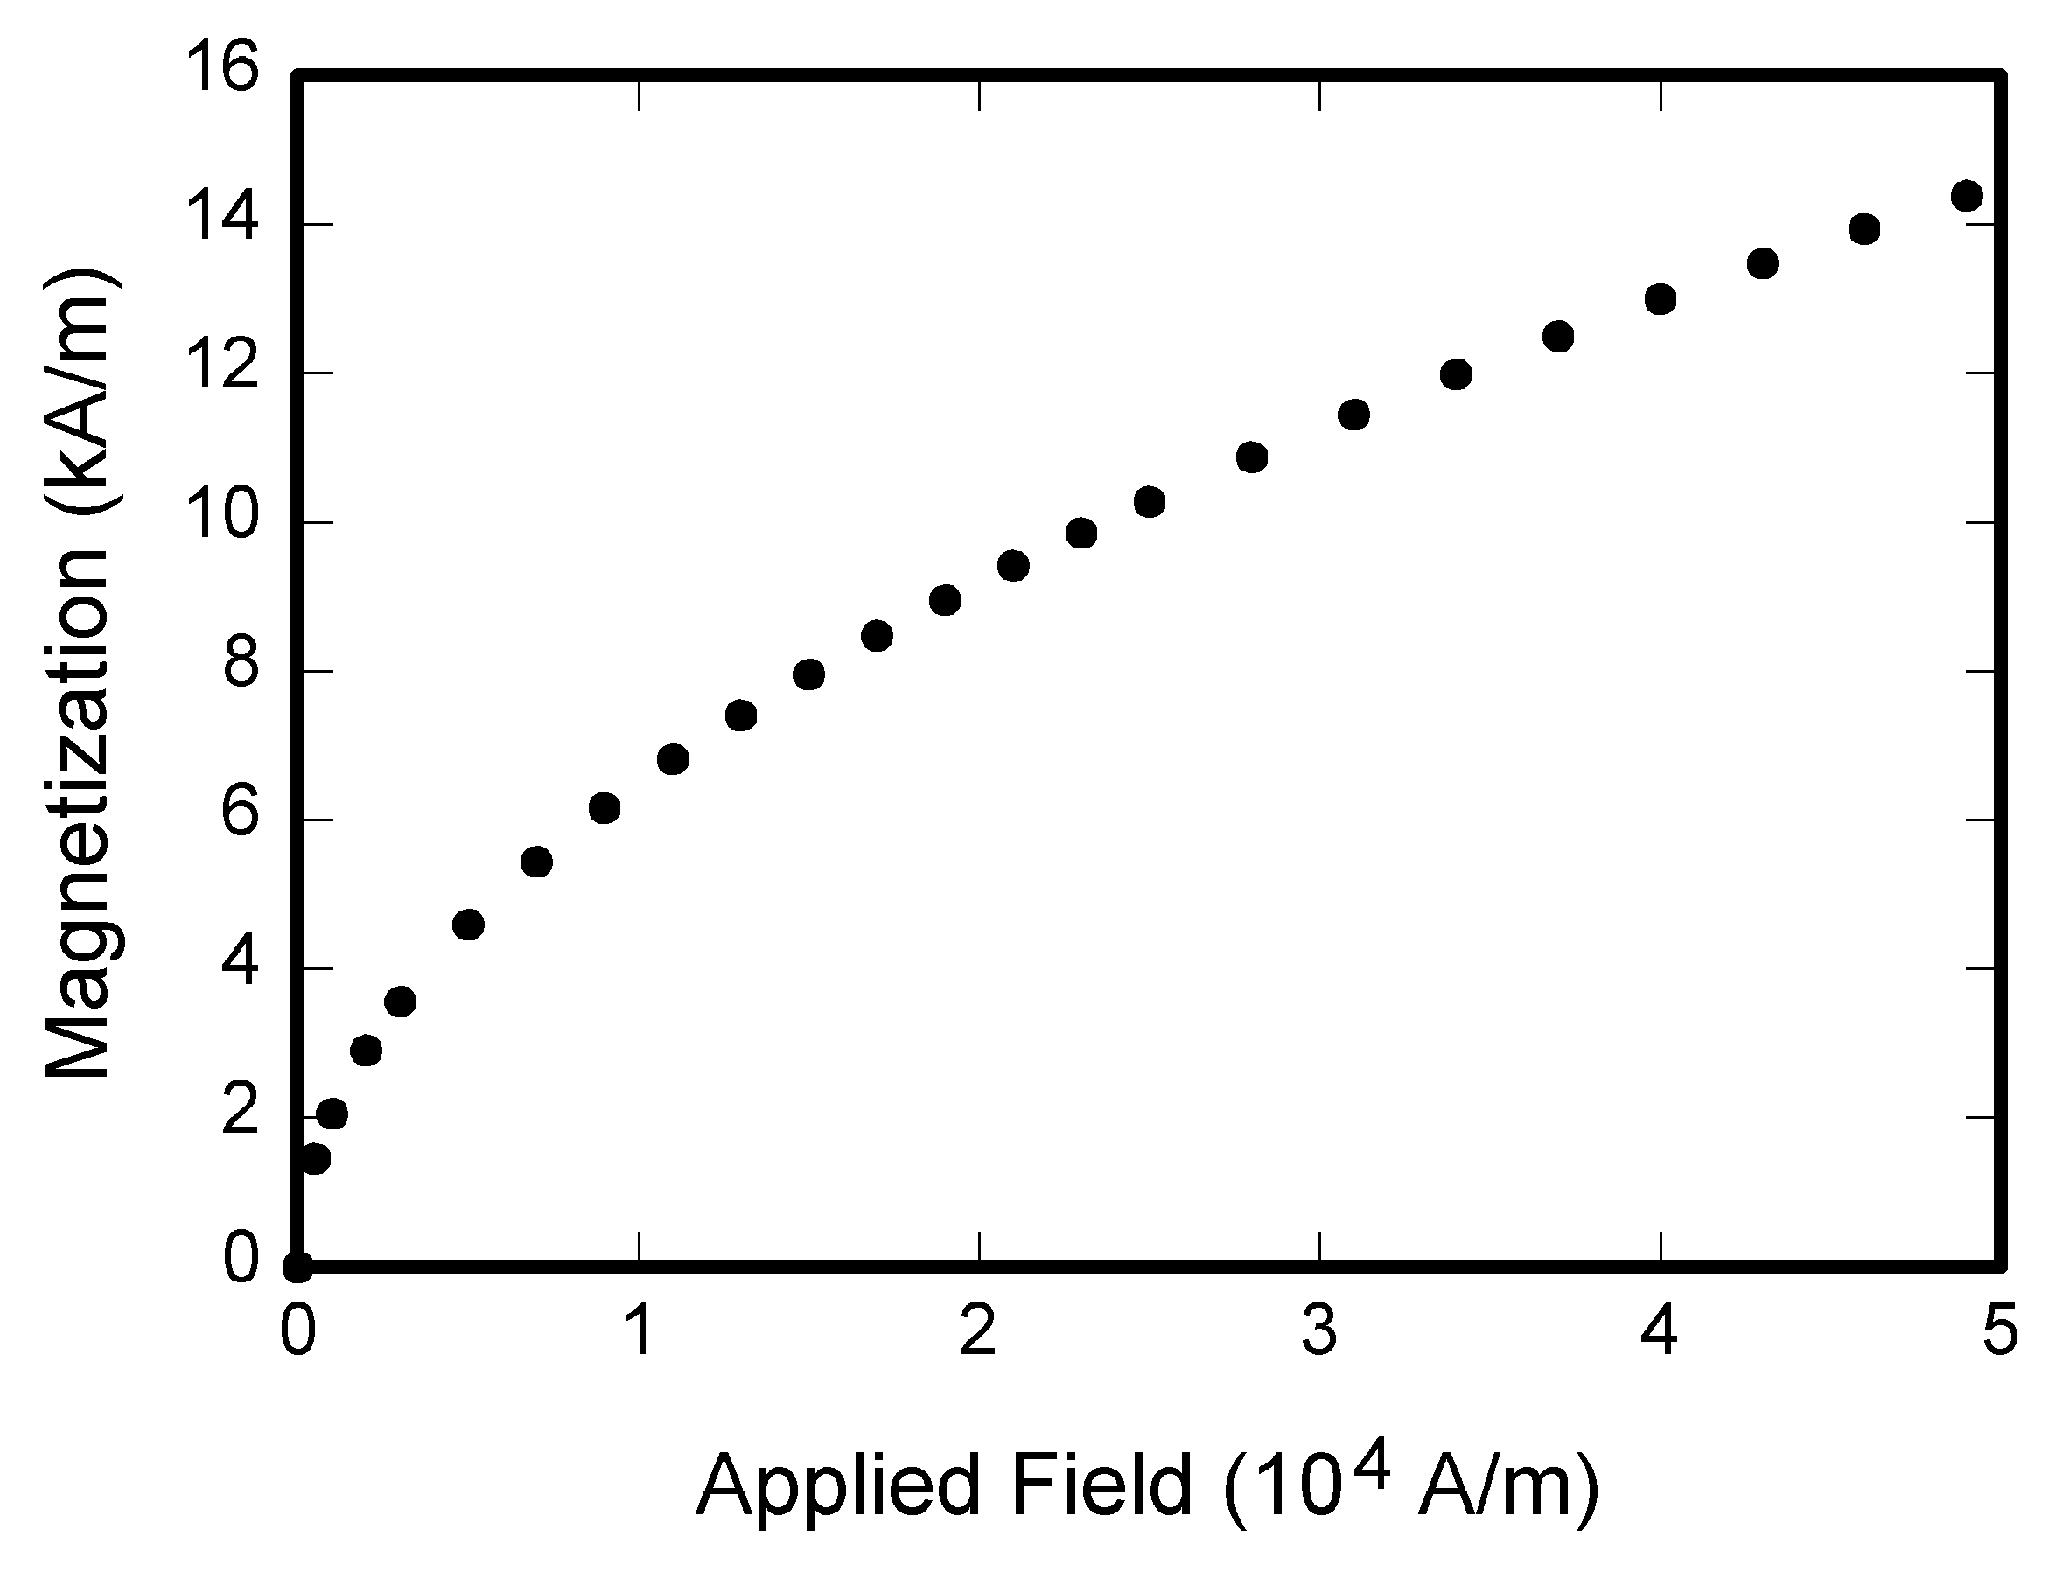
\includegraphics[width=0.7\columnwidth]{figure/image/fig1.png}}
\caption{Magnetization as a function of applied field.
It is good practice to explain the significance of the figure in the caption.}
\label{fig:fig1}
\end{figure}
\newperson{Reviewer 4}{R4}
\label{sec:R4}
\general{
XXXX.} \\
\response{
\textcolor{orange}{Thank you for XXX. }}

\question{XXXX}

\answer{\textcolor{orange}{XXXX
}}
\input{table/table}


\bibliographystyle{unsrt}
\bibliography{test}
\end{document}

